\prefacesection{Anteproyecto}
Previo al desarrollo del proyecto se describe el planeamiento que se realizó, siguiendo los lineamientos del Project Management.
\\
\begin{flushleft}
{\Large \textbf{Project charter}}
\end{flushleft}
\begin{figure}[H]
  \centering
    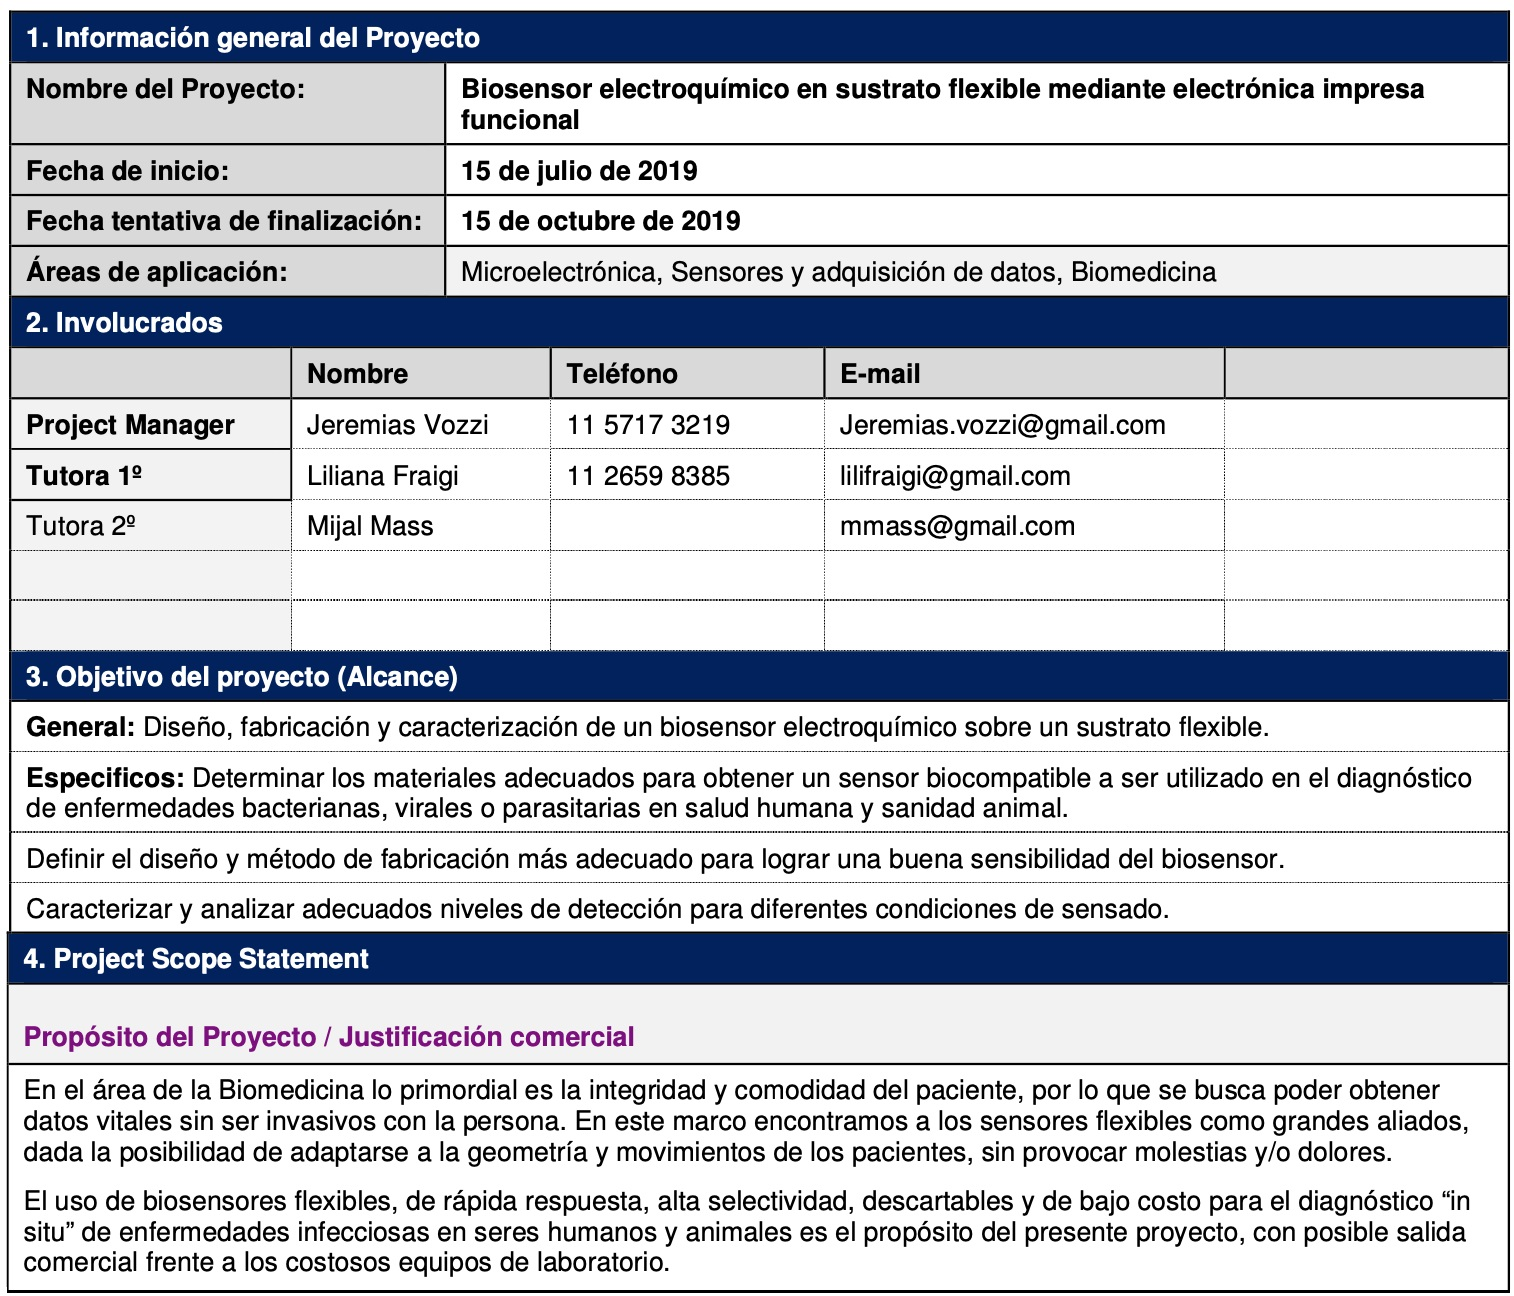
\includegraphics[width=1\textwidth]{Figuras/ProjChart1}
  \label{fig:ProjChart1}
\end{figure}
\begin{figure}[H]
  \centering
    
\includegraphics[width=1\textwidth]{Figuras/ProjChart2}
  \label{fig:ProjChart2}
\end{figure}
\begin{figure}[H]
  \centering
    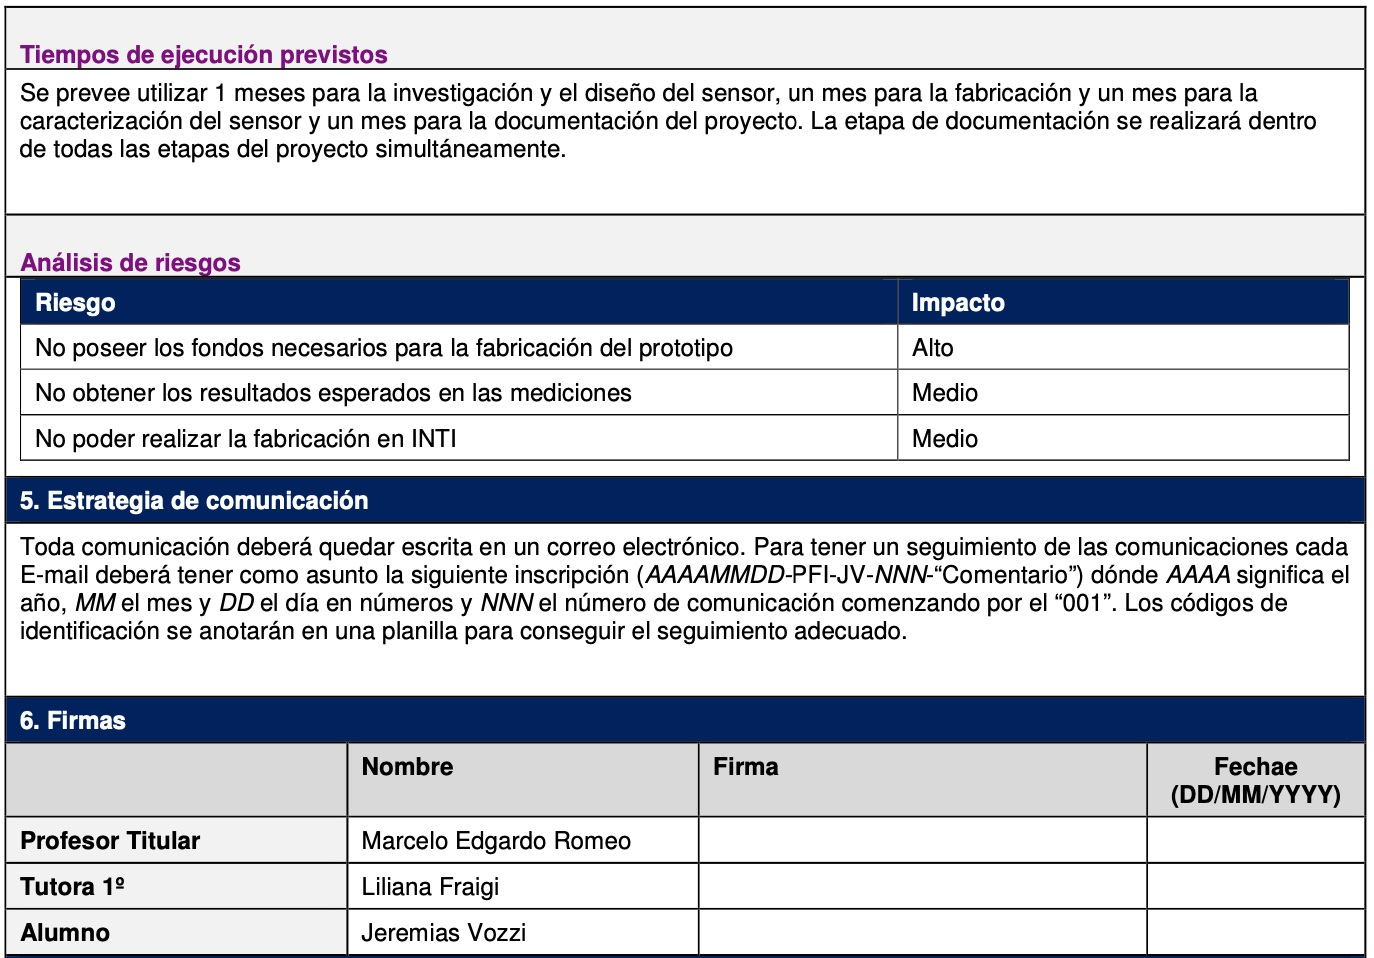
\includegraphics[width=1\textwidth]{Figuras/ProjChart3}
  \label{fig:ProjChart3}
\end{figure}
\newpage 
\begin{flushleft}
{\Large \textbf{Work breakdown structure}}
\end{flushleft}
\begin{figure}[H]
  \centering
    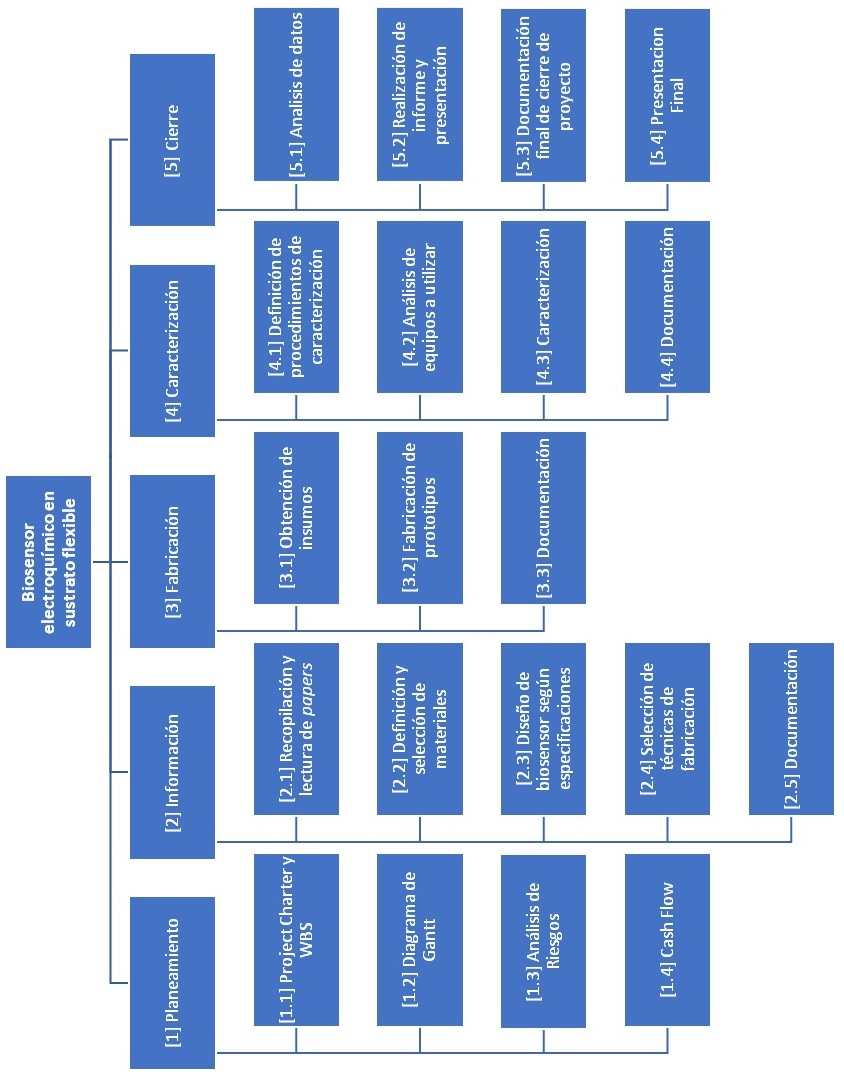
\includegraphics[width=1\textwidth]{Figuras/WBS}
  \label{fig:WBS}
\end{figure}
\newpage 
\begin{flushleft}
{\Large \textbf{Diagrama de Gantt}}
\end{flushleft}
\begin{figure}[H]
  \centering
    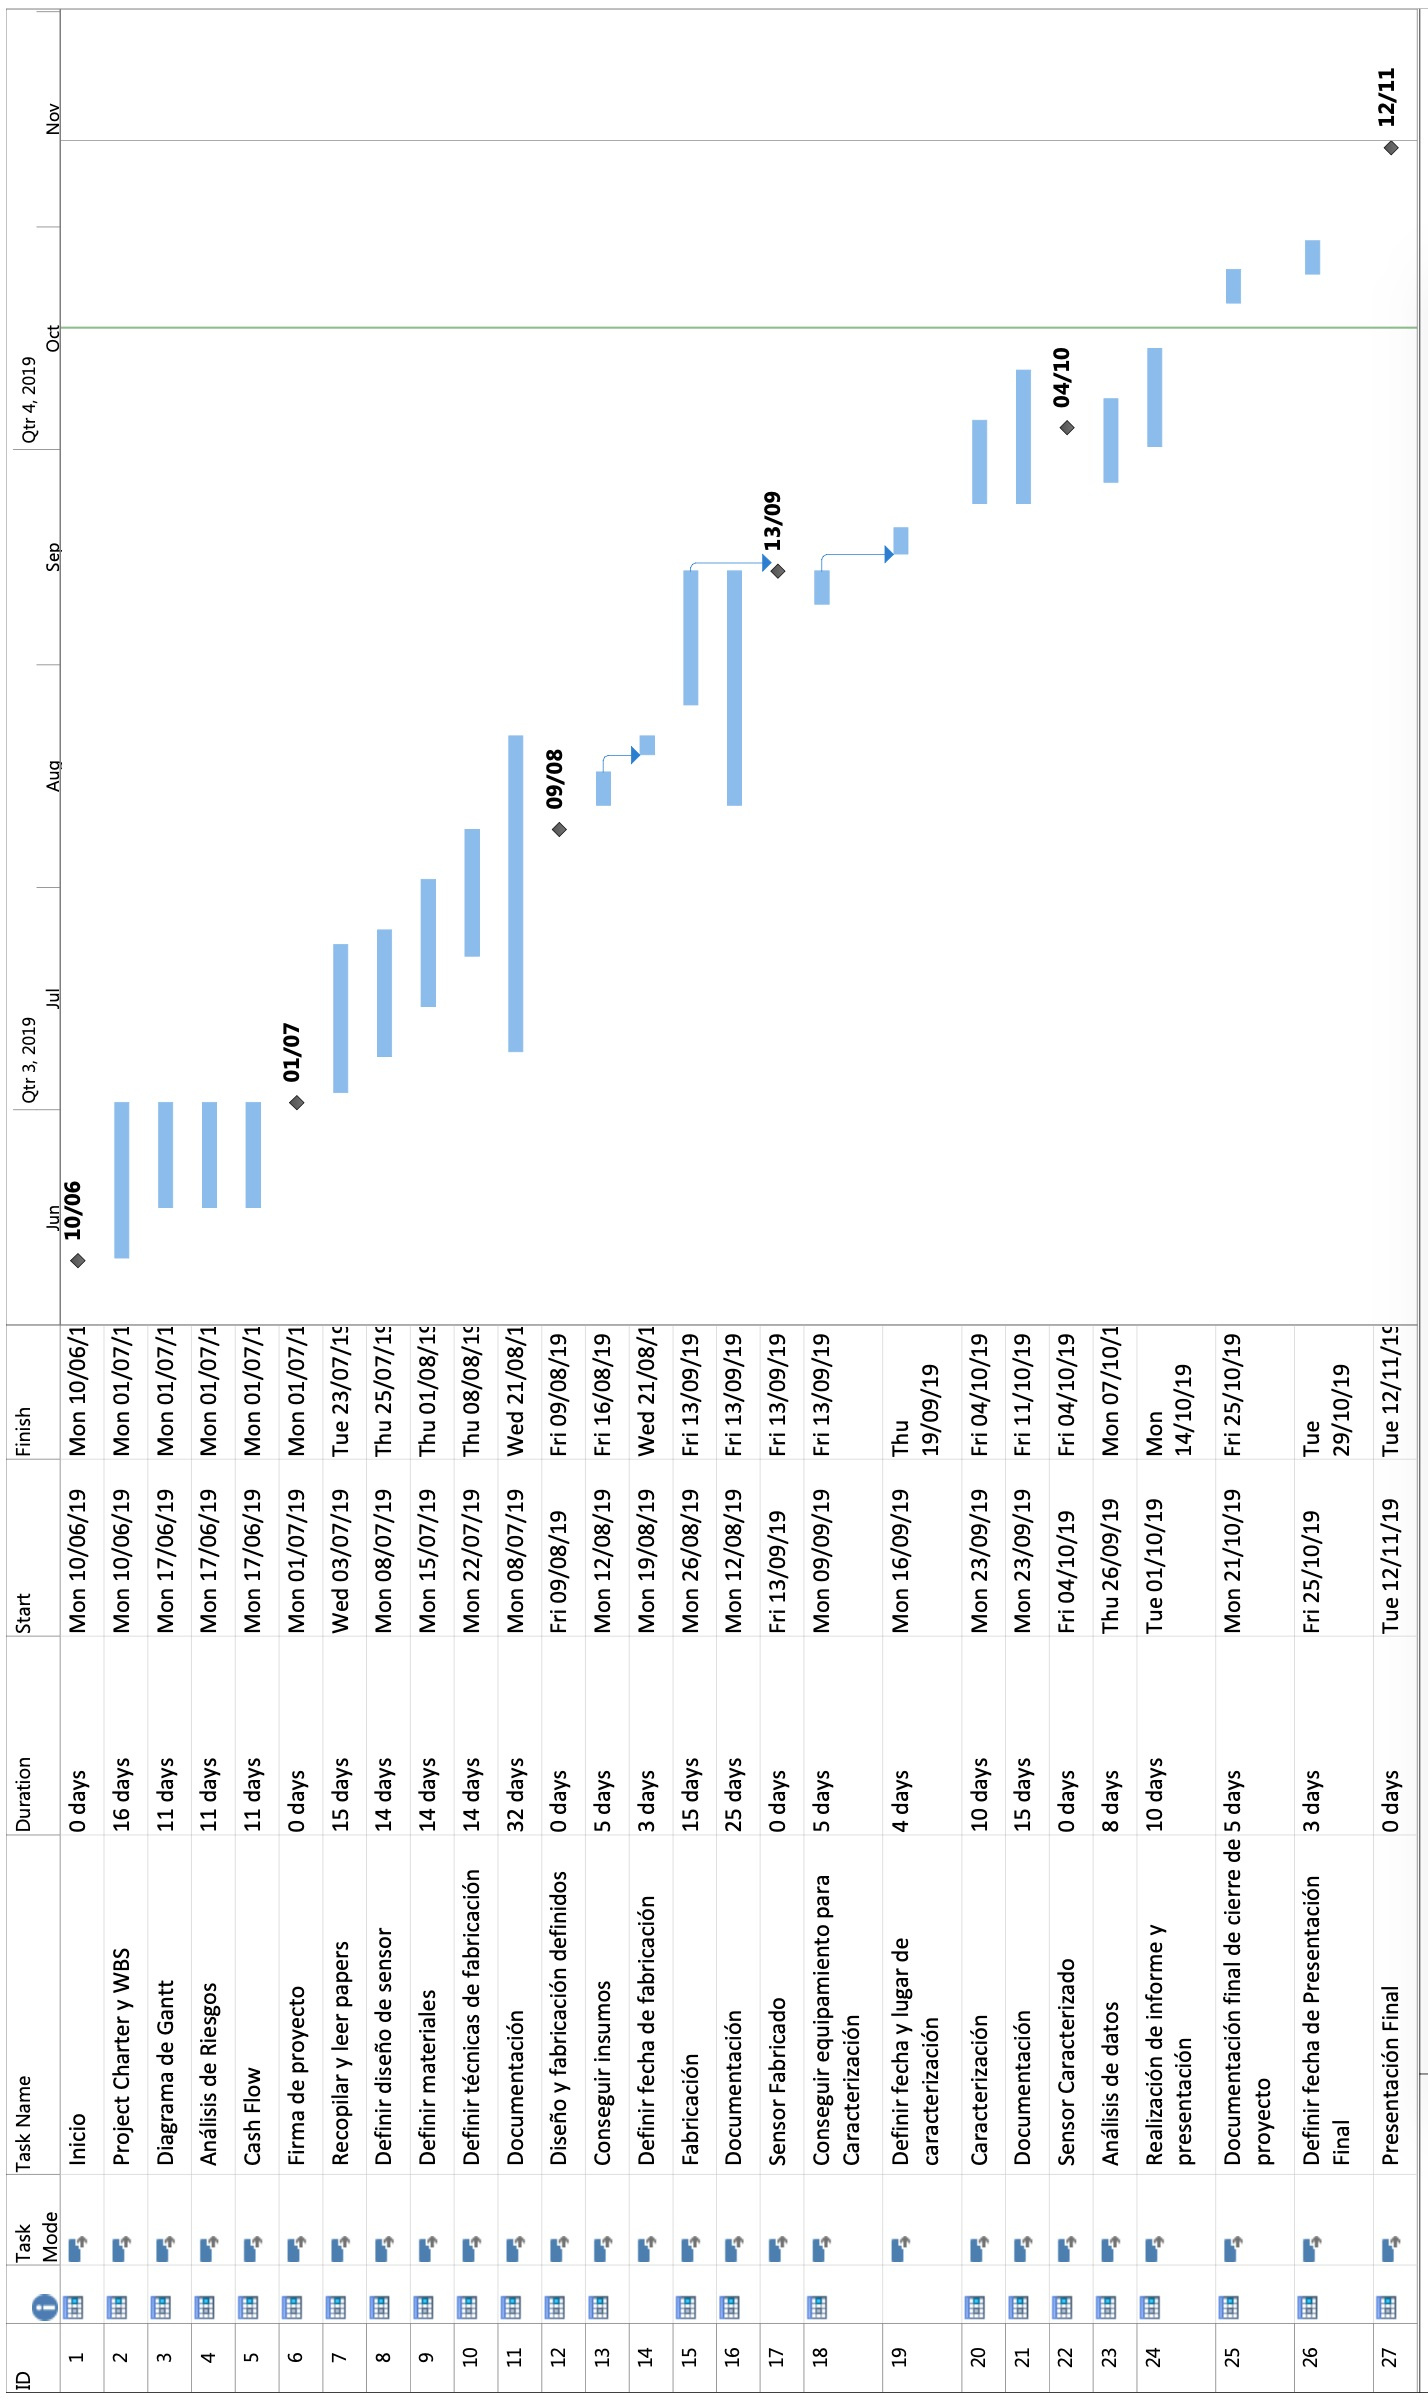
\includegraphics[width=0.82\textwidth]{Figuras/Gantt}
  \label{fig:Gantt}
\end{figure}
\newpage 
\begin{flushleft}
{\Large \textbf{Evaluación de riesgos}}
\end{flushleft}
\begin{figure}[H]
  \centering
    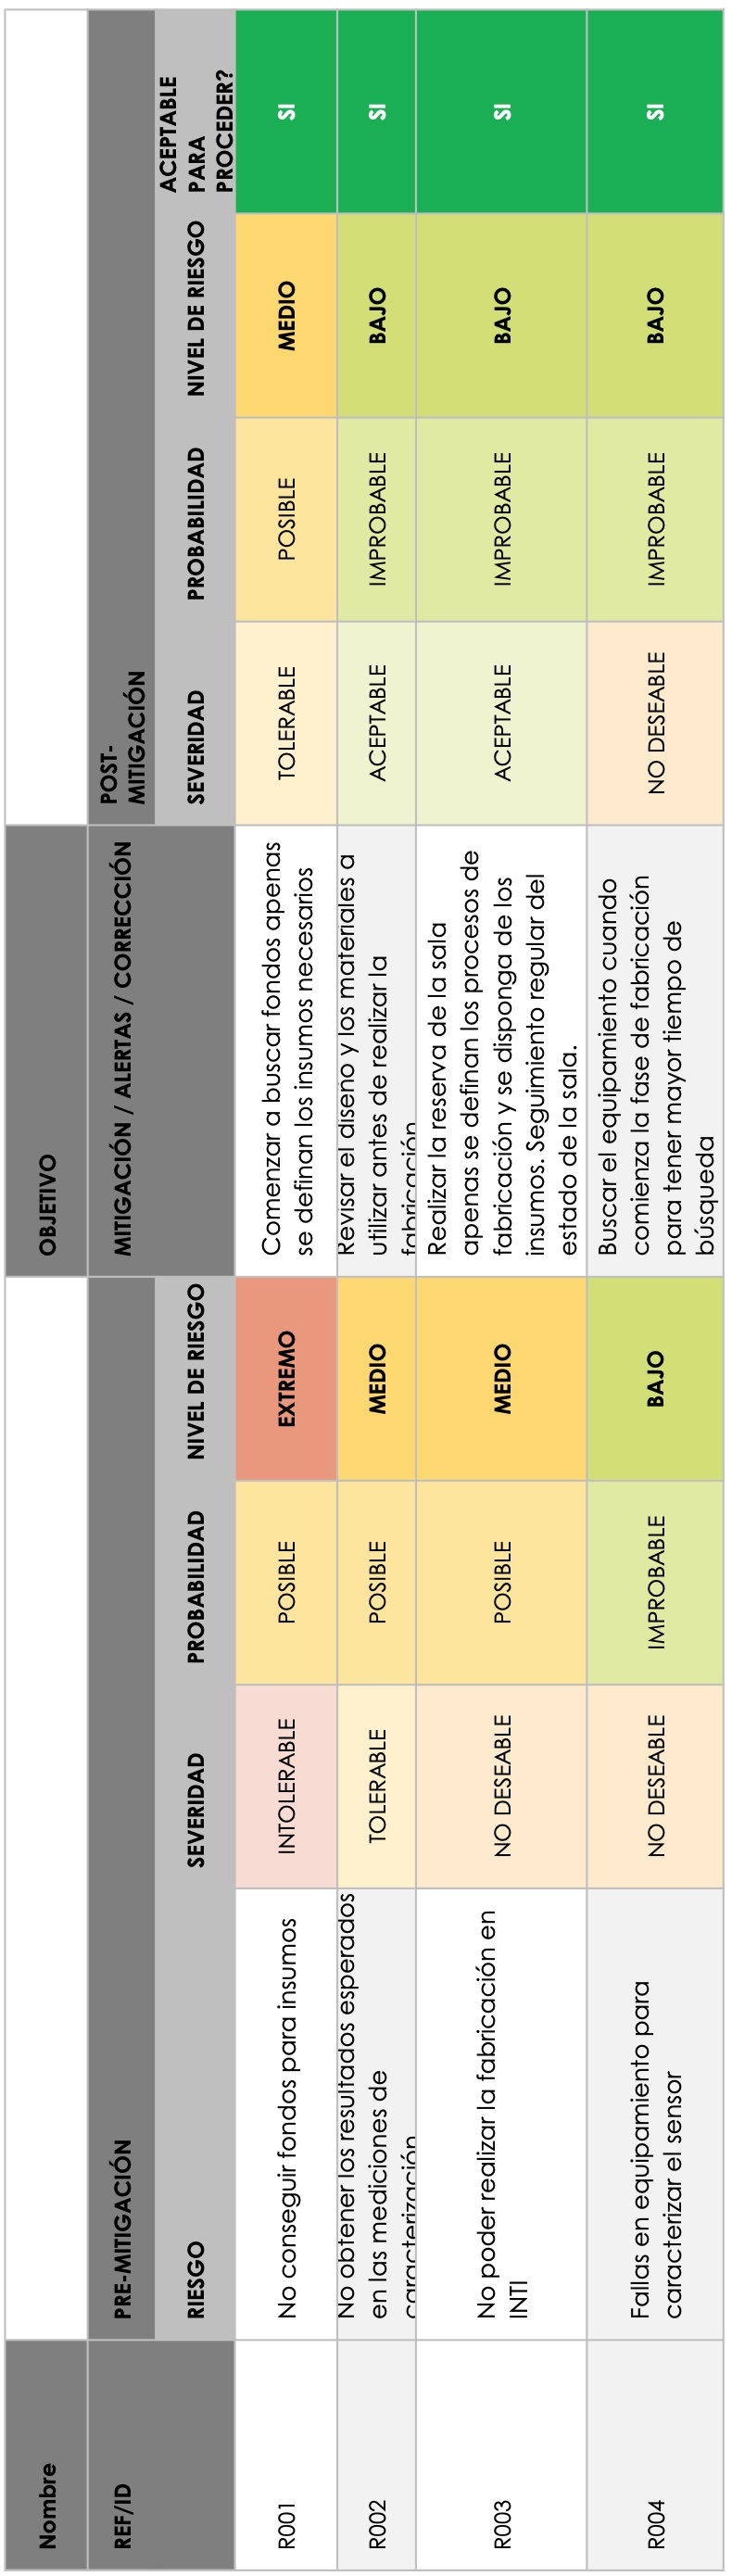
\includegraphics[width=0.38\textwidth]{Figuras/MatRiesgos}
  \label{fig:MatRiesgos}
\end{figure}
\newpage 
\begin{flushleft}
{\Large \textbf{Cashflow}}
\end{flushleft}
\begin{figure}[H]
  \centering
    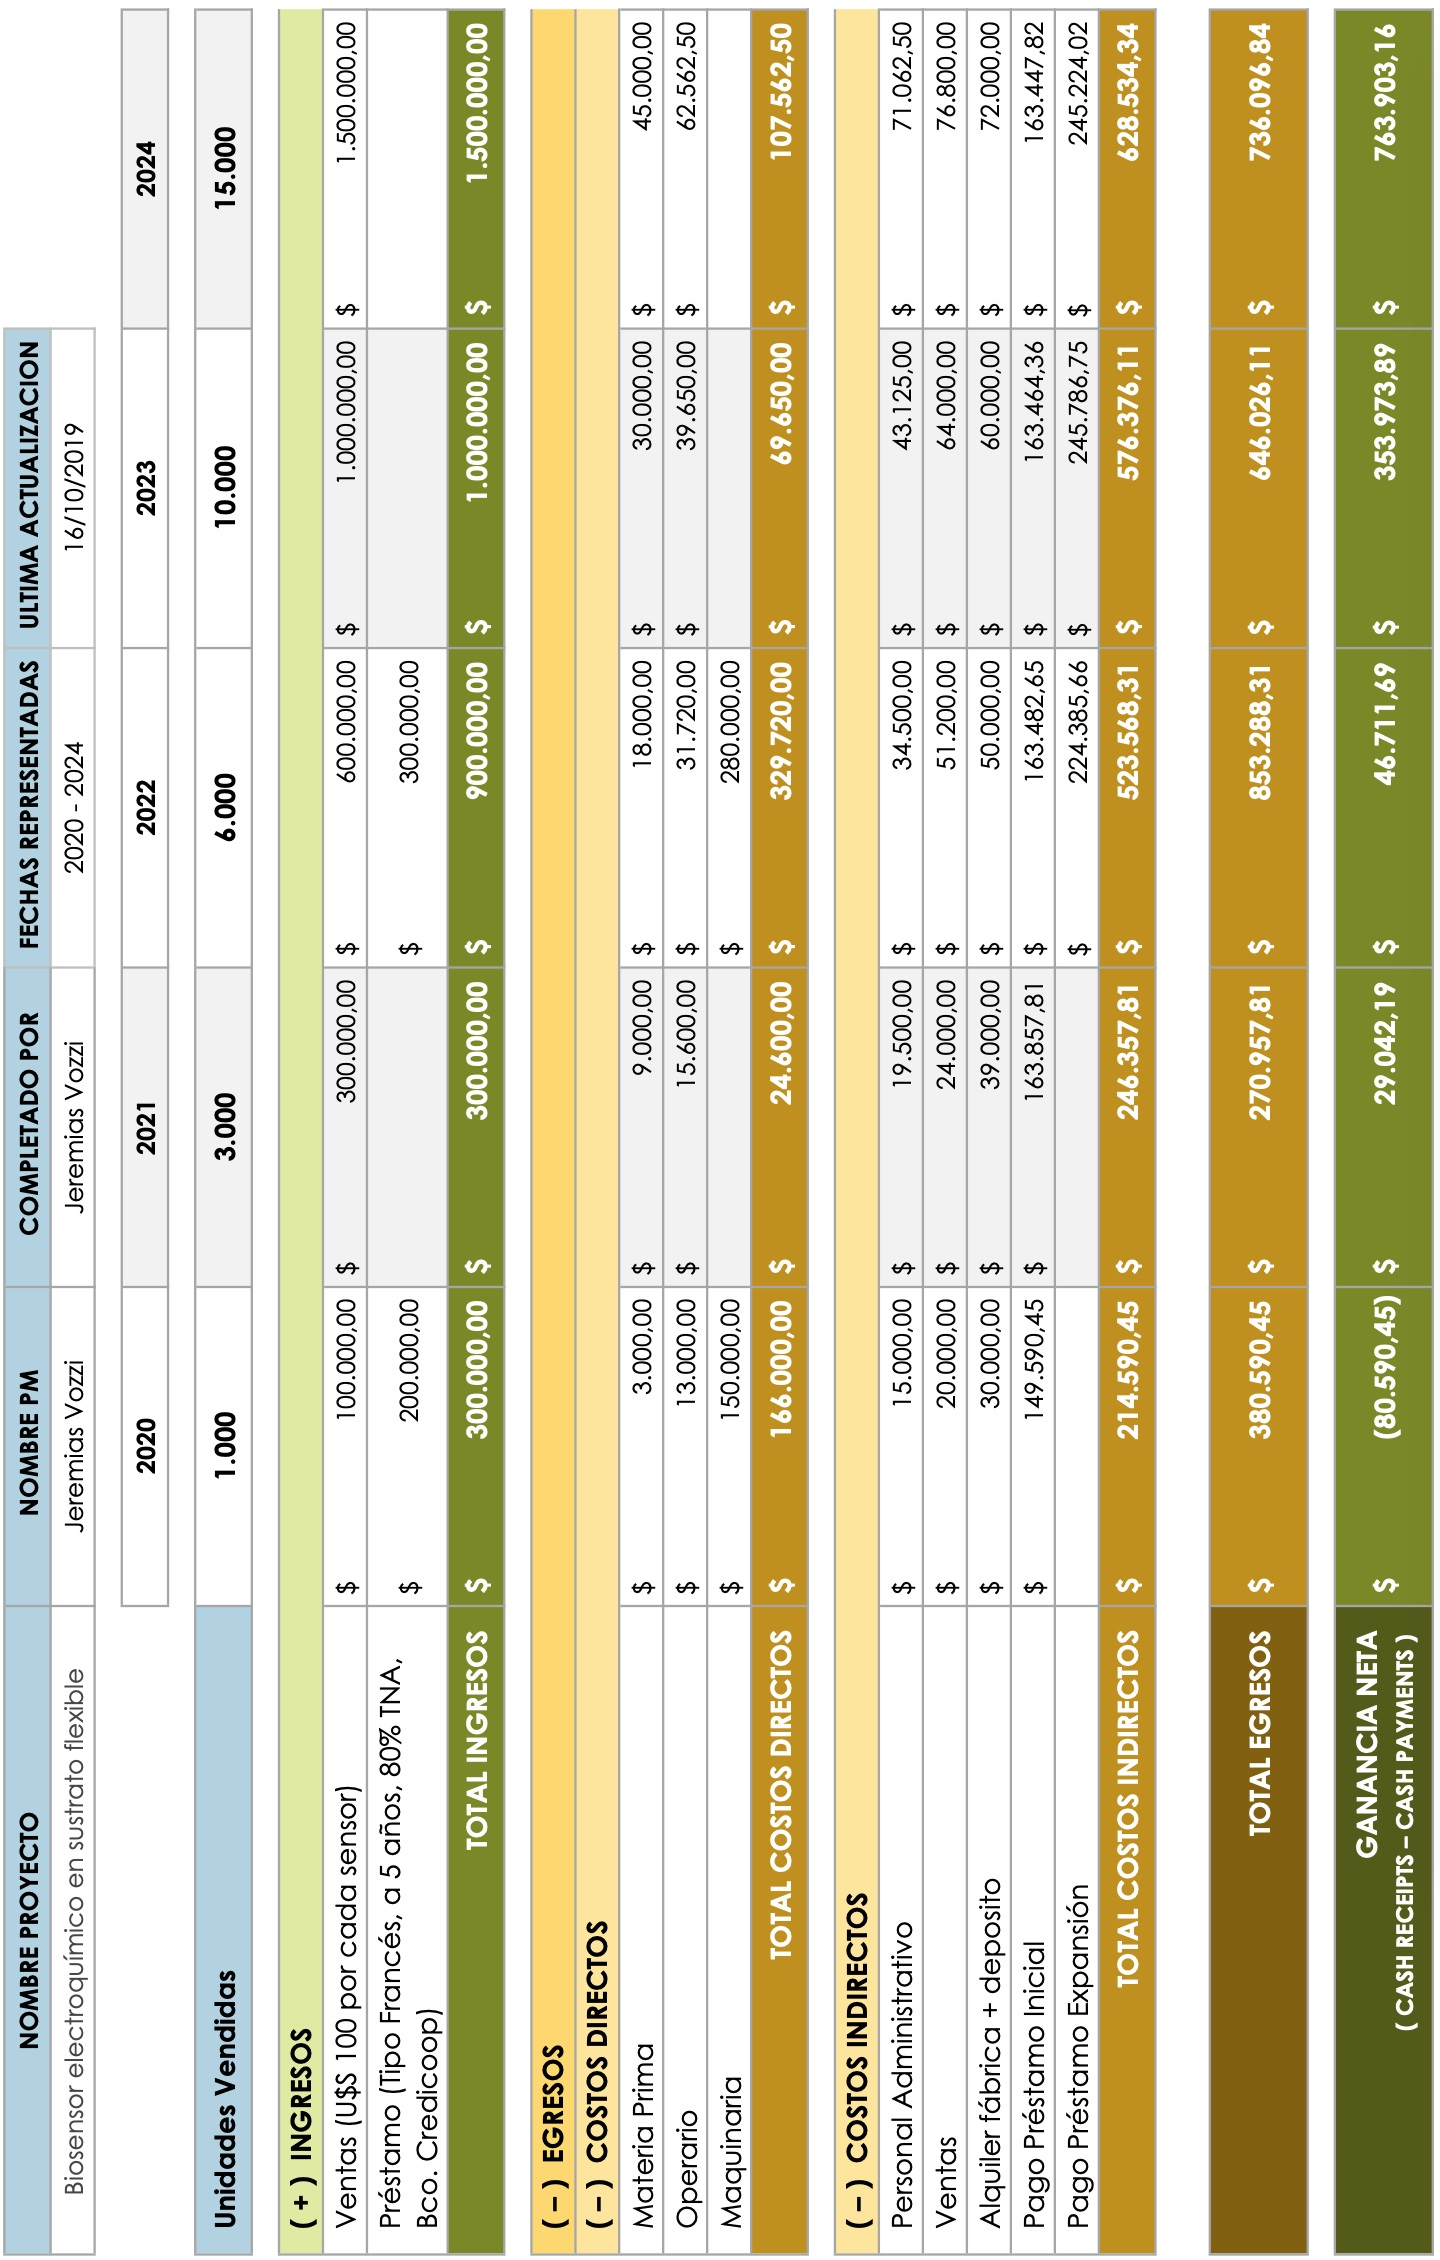
\includegraphics[width=0.85\textwidth]{Figuras/CashFlow}
  \label{fig:CashFlow}
\end{figure}

\begin{flushleft}
{\Large \textbf{Proceso de seguimiento y control}}
\end{flushleft}
Para realizar el seguimiento del proyecto se optó por generar reportes parciales sobre el estado del proyecto, una vez por semana, a través de actualizaciones de avance en el Gantt. Esto se llevo a cabo utilizando el software Project de Microsoft. De esta manera, en conjunto con los tutores, se registró el desempeño semanal teniendo en cuenta los adelantos o atrasos en las tareas y el cumplimiento de los hitos a tiempo. Mediante una reunión por semana, utilizando estos reportes, se actualizaba el cronograma y se planificaba la semana siguiente para cumplir con los objetivos propuestos.

De esta forma, se logró cumplir con los tiempos, costos y alcance estipulados.